This section presents an analysis of the microstructure based on the nearest neighbor probability density function. 
%age included nearest pair probability density function  $P_\text{nst}(\textbf{x},\textbf{r},t,a)$ and on .


%After identifying the different forms of the microstructure with respect to the dimensionless parameters, we introduce a general and concise way to quantify it.
By definition, $P_\text{nst}(\textbf{r}|\textbf{x},t)$ does not require symmetry with respect to the variable $\textbf{x}+\textbf{r}$ and \textbf{x}, as is the case for classical particle-pair distribution functions. 
Nevertheless, it turns out that $P_\text{nst}$ possesses a nearly-symmetric distribution, such that  $P_\text{nst}(r,\theta)\approx P_\text{nst}(r,- \theta)$ as demontrated below.
\begin{figure}[h!]
    \centering
    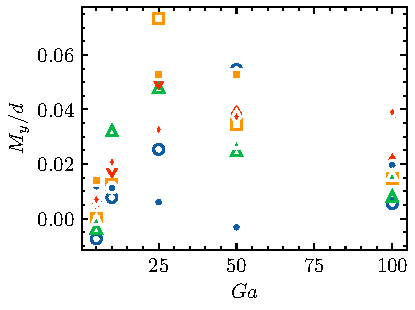
\includegraphics[height = 0.3\textwidth]{image/HOMOGENEOUS_NEW/PA/Ry.pdf}
    \caption{ Dimensionless first moment of the nearest particle pair distribution in the direction of gravity $M_y/d$. 
    ($\pmb\bigcirc$) $\phi = 0.01$; ($\pmb\triangle$) $ \phi = 0.05$; ($\pmb\square$) $\phi = 0.1$ ($\pmb\lozenge$) $\phi = 0.2$.
    The hollow symbols correspond to $\lambda = 1$, the filled symbols to $\lambda = 10$.
    % For $r<d$ we arbitrarily set $P_\text{r}^\text{th} = 1$ so that the distribution can be visualized.
    % Black symbols represent the results of \citet{zhang2023evolution} for hard sphere suspension with $\phi = 0.016,0.056,0.134,0.262$  %$\phi = 0.0168,0.0565,0.1341,0.2622$ 
    % corresponding to $\pmb\times,\pmb +, \pmb\star , \pmb\triangledown$, respectively.
    }
    \label{fig:ap:RY}
\end{figure}
%This is demonstrated by \ref{fig:ap:RY} 
%where we can see that the first moment of $P_\text{nst}$, namely
We define the first moment of $P_\text{nst}$ as
\begin{equation}
 \textbf{M} = \int_{\mathbb{R}^3} \textbf{r} P_\text{nst}(\textbf{r}) d\textbf{r}.
\end{equation}
\ref{fig:ap:RY} illustrates the projection of $\textbf{M}$ along the direction of gravity. 
The relatively small but finite values of $M_y$ indicate that $P_\text{nst}$ exhibits a nearly symmetric distribution with respect to $\theta$.
Nevertheless, this indicates that the nearest neighbor is more likely to be located in the upstream direction. 
Note that this is consistent with the findings of \citet{zhang2023evolution}.
Even though this slight asymmetry might have its importance \cite{zhang2023evolution}, we discard it in this study. 
Therefore, we choose to show only the upper part of the distribution in the following plots, (displayed in \ref{fig:Pnst_low_Ga} and \ref{fig:Pnst_high_Ga}) since qualitatively it remains the same as the lower part.  
Additionally, in the discussion below, we refer to the sphere at the origin of the graphs, located at $\textbf{x}=0$, as the \textit{test particle}.%\textit{test particle} or the \textit{test particle}. 

\subsection{Low inertia regimes}
We begin with a detailed analysis of $P_\text{nst}$ at $Ga =10$, to investigate the influence of $\lambda$ and $\phi$ on the microstructure when inertial effects are small.
\begin{figure}[h!]
    \centering
    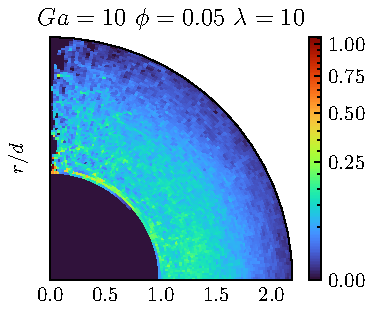
\includegraphics[height=0.21\textwidth]{image/HOMOGENEOUS_NEW/Dist/Pnst_l_10_Ga_10_PHI_0_05.pdf}
    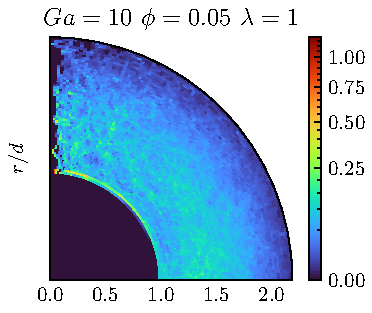
\includegraphics[height=0.21\textwidth]{image/HOMOGENEOUS_NEW/Dist/Pnst_l_1_Ga_10_PHI_0_05.pdf}
    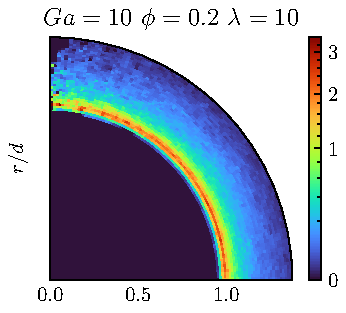
\includegraphics[height=0.21\textwidth]{image/HOMOGENEOUS_NEW/Dist/Pnst_l_10_Ga_10_PHI_0_2.pdf}
    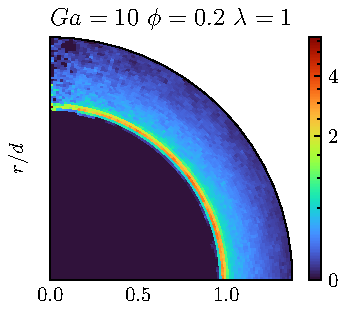
\includegraphics[height=0.21\textwidth]{image/HOMOGENEOUS_NEW/Dist/Pnst_l_1_Ga_10_PHI_0_2.pdf}
    \caption{Histogram of the probability density function, $P_\text{nst}(r,\theta)$, for low inertia $Ga = 10$.
    The color map represents the nearest pair distribution function. %the values of $P_\text{nst}$.
    The origin corresponds to the position of the \textit{test particle}.
    The dimensionless radial and azimuthal coordinates, $|\textbf{r}|/d$ and $\theta$, correspond to the nearest neighbor position.
    The vertical direction corresponds to the flow direction, which is also the axis of symmetry for $P_\text{nst}$.
    (left) Low volume fraction cases $\phi=0.05$ for $\lambda = 1,10$.
    (right) High volume fraction cases $\phi=0.2$ for $\lambda = 1,10$.
    }
    \label{fig:Pnst_low_Ga}
\end{figure}
The first observation from \ref{fig:Pnst_low_Ga} indicates that the likelihood of finding the nearest neighboring particle at an angle $\theta$ is uniform across all $\theta$.
This suggests that $P_\text{nst}$ is isotropic at these \textit{Galileo} numbers. We can observe that $P_\text{nst}$ is larger close to the \textit{test particle} ($r/d = 1$) in the high volume fraction cases than in the low volume fraction cases.
%If we compare the low volume fraction cases to the high volume fraction cases, we can observe that $P_\text{nst}$ is larger at near contact of the test particle ($r/d = 1$) in the latter case.
% For solid particles it is also common that pair distributions are more concentrated at the contact of the test particle for increasing $\phi$. 
In practice, if particles are more likely to be close to one another, it means that densely packed regions of particles are present in the flow.
This suggests that isotropic clusters, as represented in \ref{fig:scheme_clusters} (\textit{Case 2}), are likely to form in the present context. 
Regarding the effect of the viscosity ratio, $P_\text{nst}$ are very similar for both values of $\lambda$ except that for the highest volume fraction the region of highest probability is thinner for the lowest aspect ratio. 
Consequently, in this regime we find homogeneous microstructures at low $\phi$, and non-homogeneous but still isotropic microstructure (\textit{``clusters''}) at higher $\phi$. 

